\begin{exercice}[Quelques partages]
Pour chaque figure, indique la fraction de la surface totale qui est colorée :
\begin{colenumerate}{3}
 \item 
 
 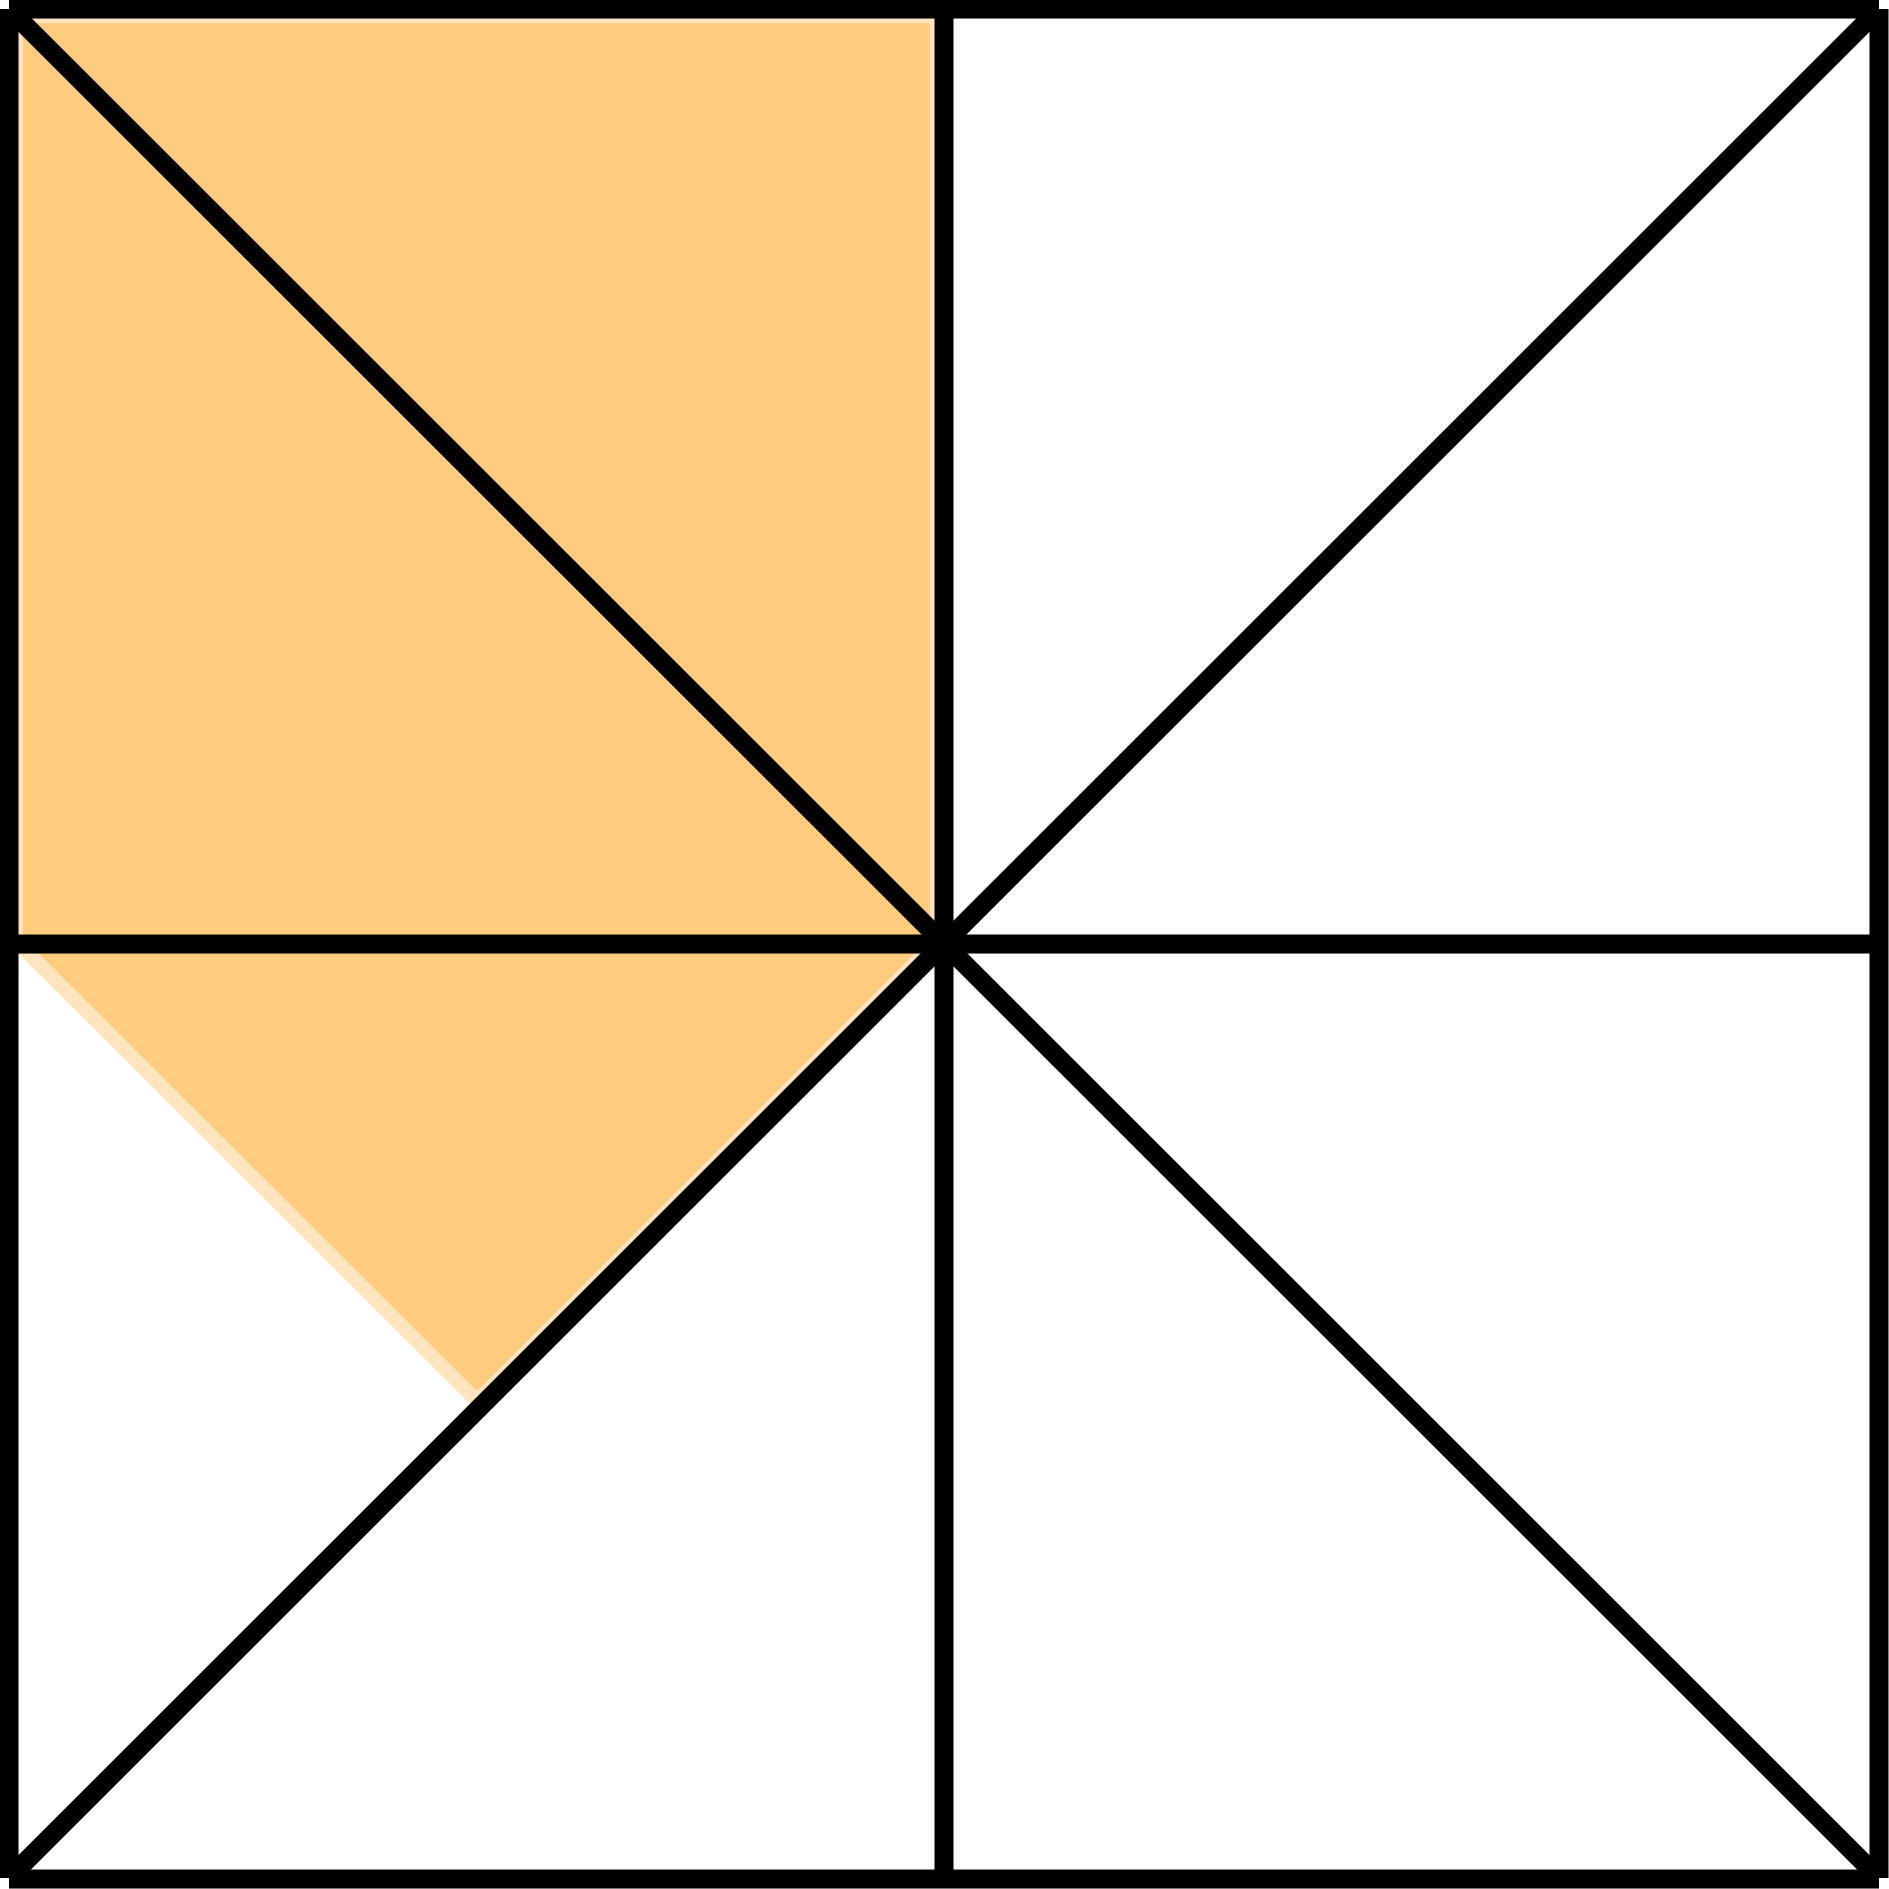
\includegraphics[width=2cm]{partages_colores}
 \item
  
 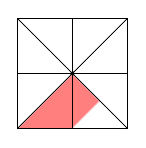
\includegraphics[width=2cm]{partages_colores2}
 \item
  
 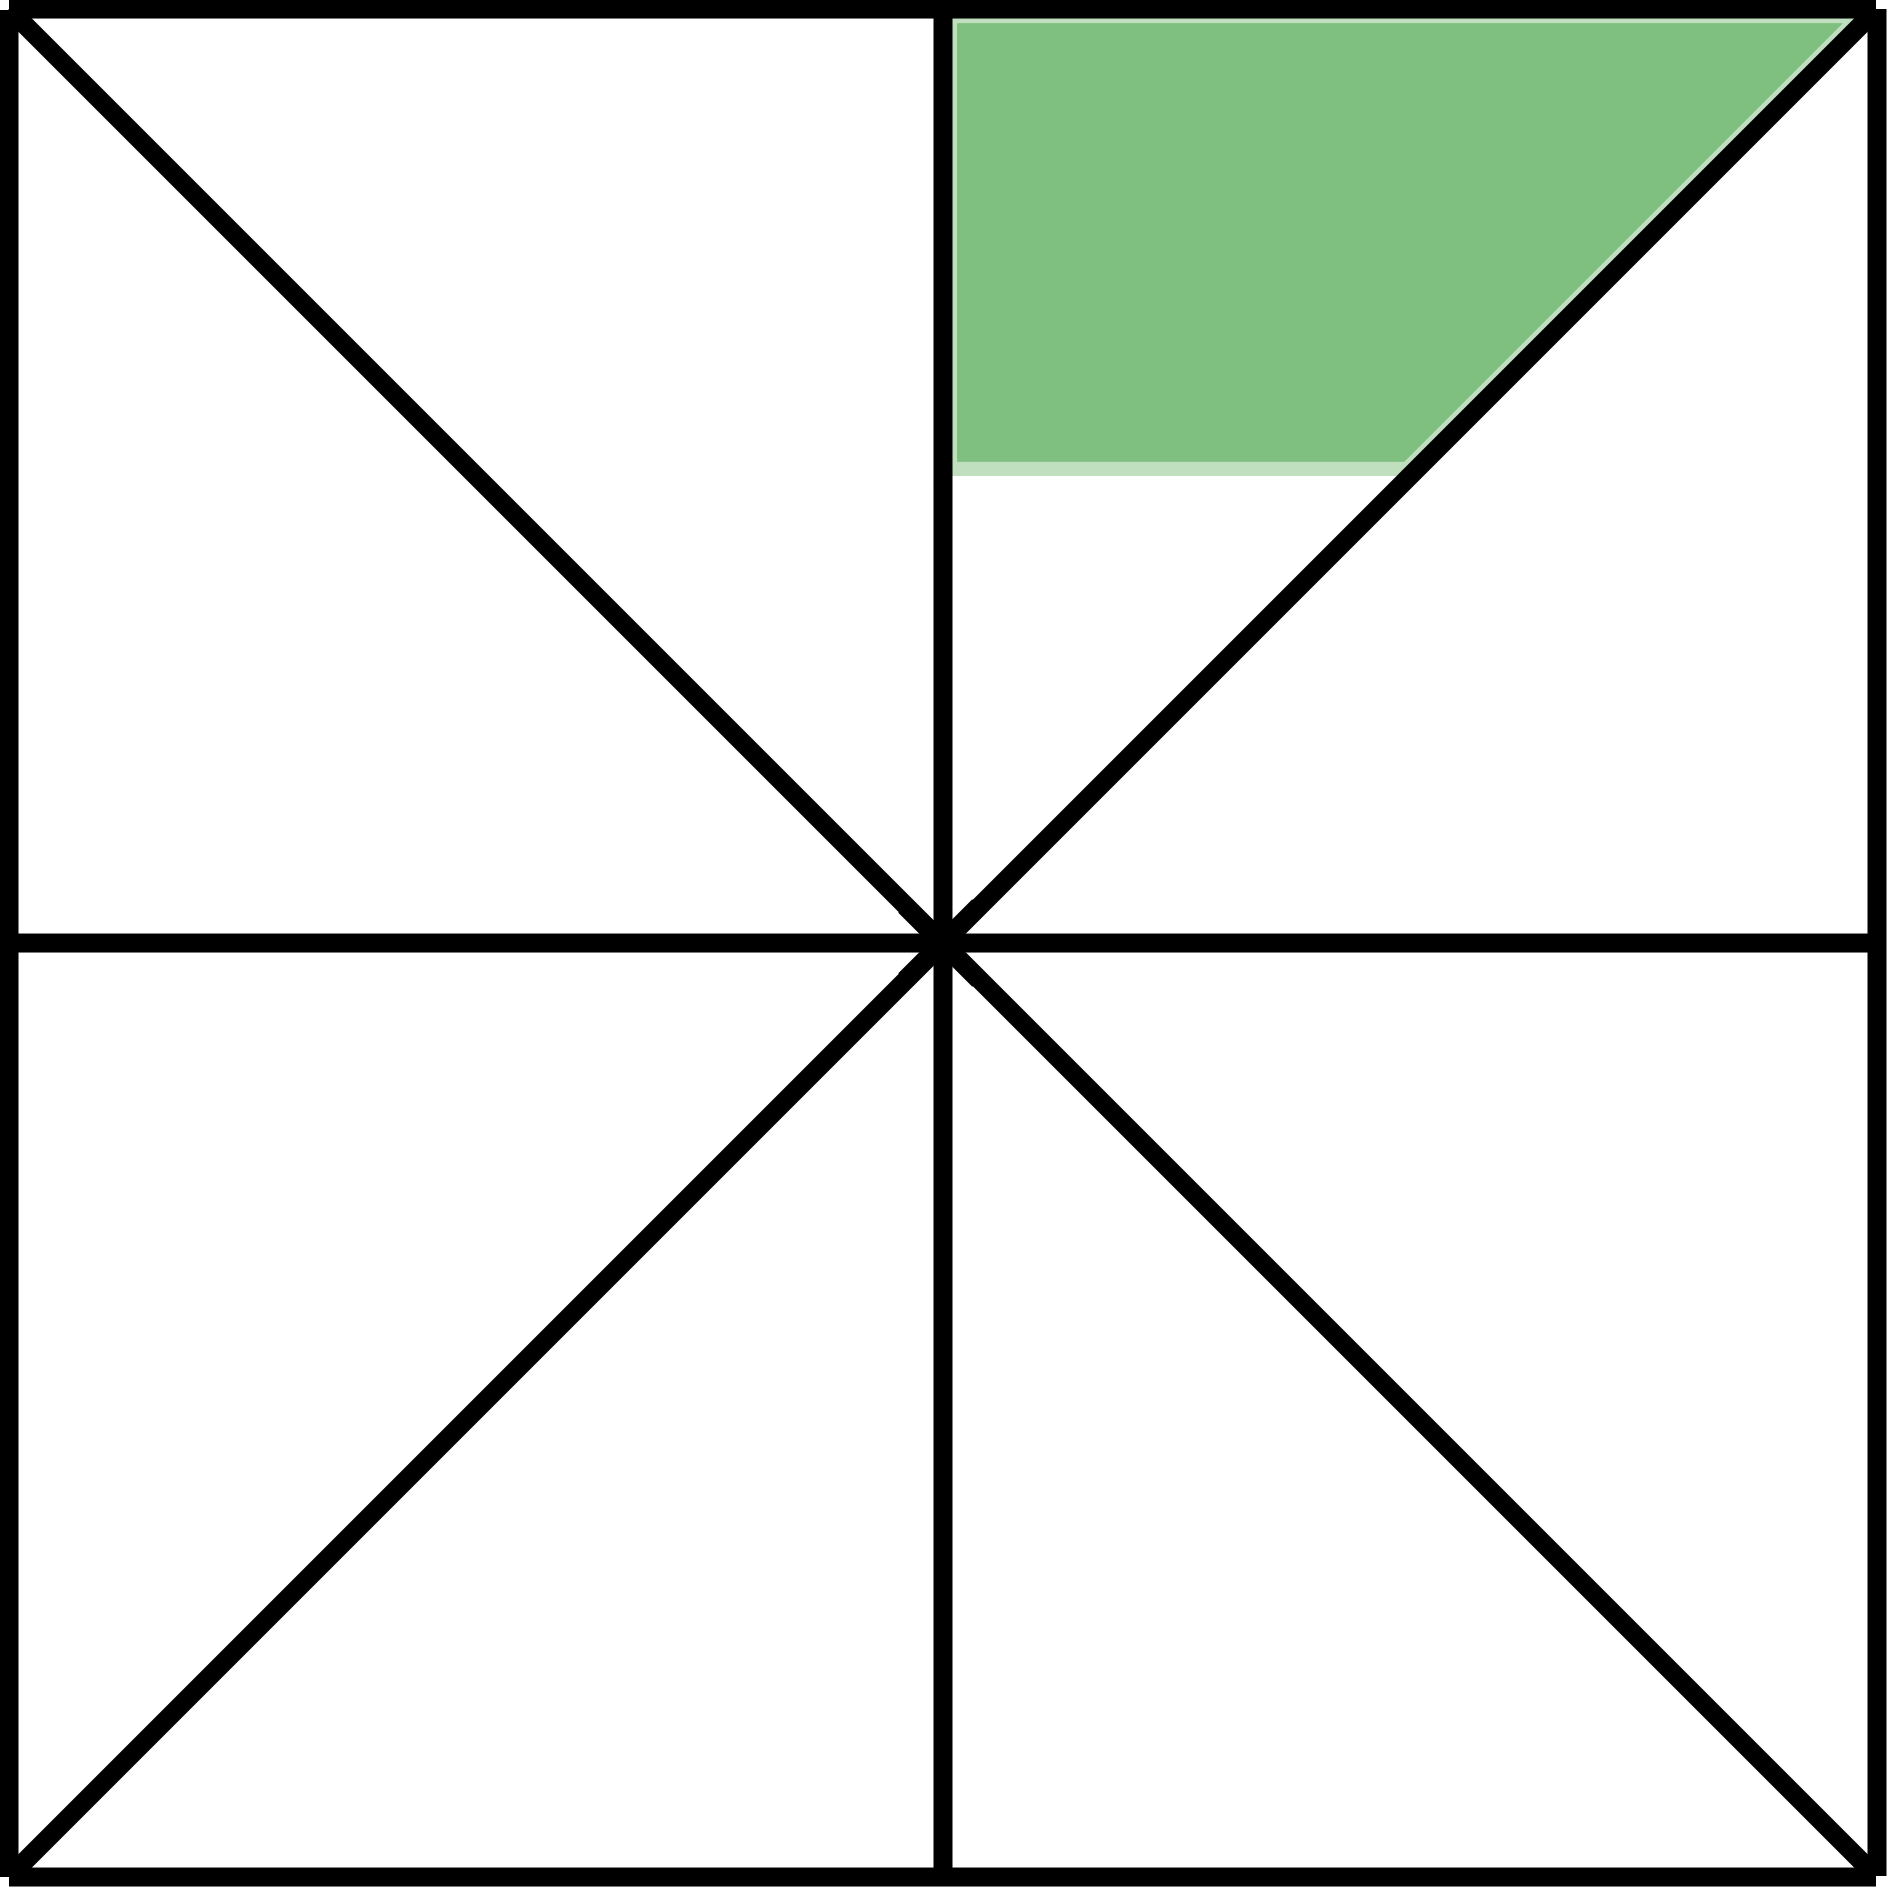
\includegraphics[width=2cm]{partages_colores3}
 \end{colenumerate}
\end{exercice}


\begin{exercice}[Coloriage]
Trace trois rectangles de 9 cm sur 4 cm.
\begin{enumerate}
 \item Partage le premier pour colorier les cinq sixièmes de sa surface ;
 \item Partage le second pour colorier les sept douzièmes de sa surface ;
 \item Partage le troisième pour colorier les trois huitièmes de sa surface.
 \end{enumerate}
\end{exercice}


\begin{exercice}
Transforme les nombres suivants en écriture décimale puis entoure d’une même couleur ceux qui sont égaux :
\begin{center}
\renewcommand{\arraystretch}{2}
  \begin{tabular}{|c|c|c|c|c|c|} 
  \hline
  \rowcolor{F2} $7 + \dfrac{1}{4}$ & 2 & $\dfrac{29}{4}$ & $\dfrac{156}{78}$ & $\dfrac{84}{10}$ & 29,4 \\\hline
  \rowcolor{F2} $8 - \dfrac{3}{4}$ & 8,4 & $\dfrac{8}{4}$ & $8 + \dfrac{4}{10}$ & $\dfrac{147}{5}$ & 7,25 \\\hline
  \end{tabular}
  \renewcommand{\arraystretch}{1}
 \end{center}
\end{exercice}


\begin{exercice}[À la chasse aux décimaux]
\begin{enumerate}
 \item Parmi les fractions suivantes, lesquelles sont des nombres décimaux ?
 \begin{colitemize}{4}
  \item $A = \dfrac{1}{2}$ ;
  \item $B = \dfrac{1}{3}$ ;
  \item $C = \dfrac{1}{7}$ ;
  \item $D = \dfrac{1}{10}$ ;
  \item $E = \dfrac{1}{13}$ ;
  \item $F = \dfrac{1}{25}$ ;
  \item $G = \dfrac{1}{16}$ ;
  \item $H = \dfrac{1}{12}$ ;
  \item $I = \dfrac{1}{4}$ ;
  \item $J = \dfrac{1}{15}$.
  \end{colitemize}
Tu pourras utiliser un tableau pour présenter tes résultats.
 \item Donne deux fractions de numérateur 1 (différentes des fractions ci-dessus) : une  décimale et une non décimale.
 \item Quelles remarques peux-tu faire concernant les fractions décimales ?
 \item Sans calculer les quotients, indique si les fractions suivantes sont décimales ou non, en justifiant ta réponse : $\dfrac{1}{125}$ ; $\dfrac{1}{40}$ ; $\dfrac{1}{6}$ et $\dfrac{1}{35}$.
 \vspace{0.2cm}
 \item Soulimane affirme que toute fraction décimale peut s'écrire avec un dénominateur égal à 10, 100, 1\,000 \ldots
 
 Est-ce vrai ?
 \end{enumerate}
\end{exercice}


\begin{exercice}[Demi‑droites graduées]
\begin{enumerate}
 \item Quelles sont les abscisses respectives des points $A$, $B$, $C$ et $D$ ?
 
 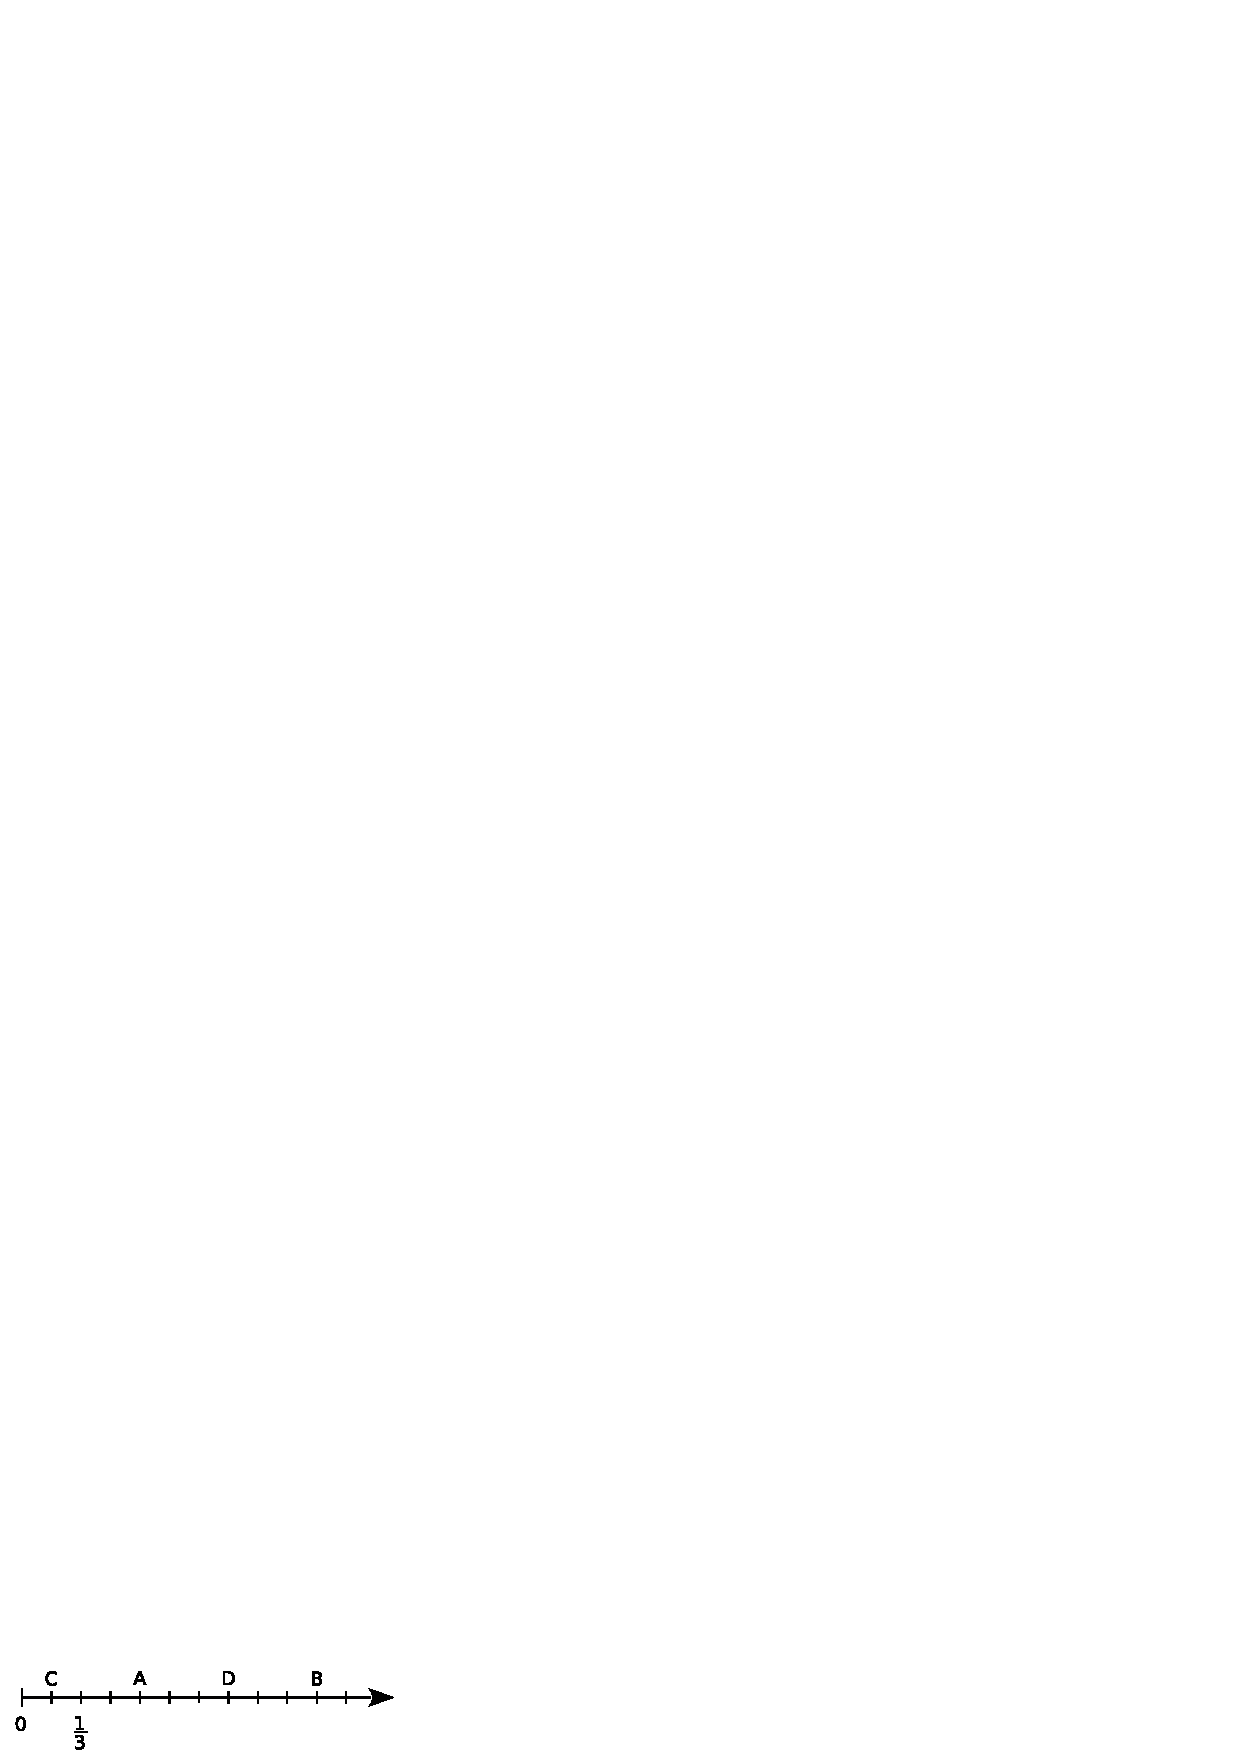
\includegraphics[width=6.7cm]{dd_fraction1}
 \item Même question pour les points $E$, $F$, $G$ et $H$.
 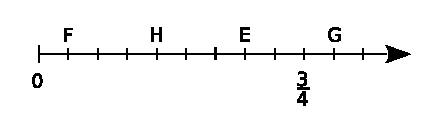
\includegraphics[width=6.7cm]{dd_fraction2}
 \item Même question pour les points $I$, $J$, $K$ et $L$.
 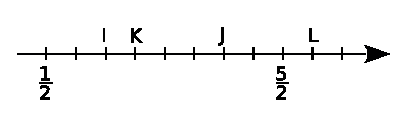
\includegraphics[width=6.7cm]{dd_fraction3}
 \item Même question pour les points $P$, $M$ et $N$.
 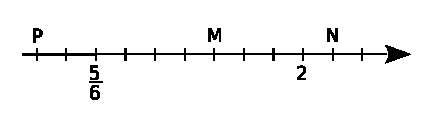
\includegraphics[width=6.7cm]{dd_fraction4}
 \end{enumerate}
\end{exercice}


\begin{exercice}
En choisissant judicieusement une unité de longueur, place précisément sur une demi‑droite graduée les points $A$ d'abscisse $\dfrac{5}{6}$, $B$ d'abscisse $\dfrac{1}{2}$, C d'abscisse $\dfrac{11}{6}$, D d'abscisse $\dfrac{3}{4}$ et E d'abscisse $1 + \dfrac{1}{3}$.
\end{exercice}


\begin{exercice}[Encore une demi‑droite graduée]
\begin{enumerate}
 \item Reproduis la demi‑droite graduée ci‑dessous en prenant trois centimètres pour unité :
 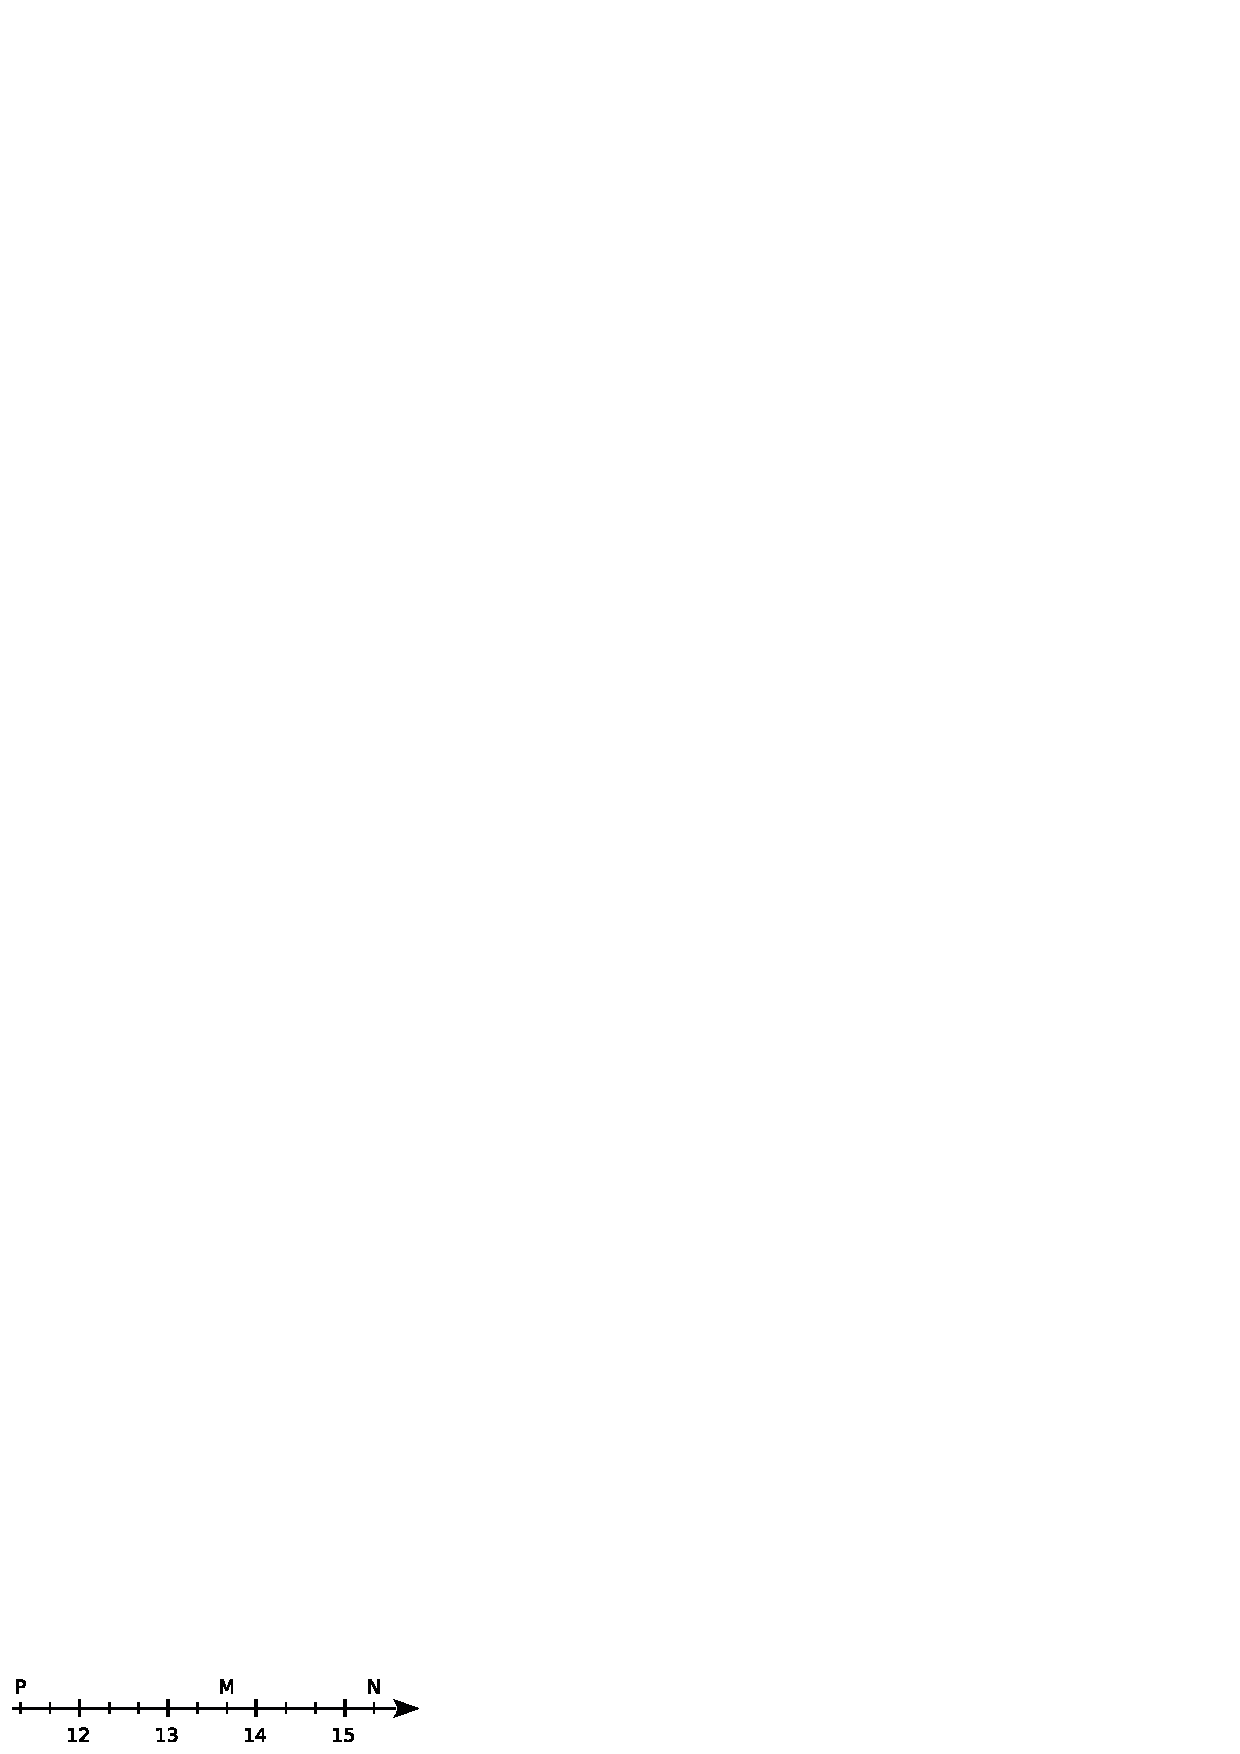
\includegraphics[width=6.7cm]{dd_PMN}
 \item Donne deux écritures de chacune des abscisses des points $M$, $N$ et $P$.
 \item Sur la demi‑droite graduée, place le point $Q$ d'abscisse $14 + \dfrac{1}{3}$, le point $R$ d'abscisse $13 - \dfrac{1}{6}$ et le point $S$ d'abscisse $\dfrac{71}{6}$.
 \end{enumerate}
\end{exercice}


\begin{exercice}[Le Scrabble\up{®}]
Le tableau suivant donne le nombre de jetons correspondant à chaque lettre de l'alphabet :
\begin{center}
\renewcommand*\tabularxcolumn[1]{>{\centering\arraybackslash}m{#1}}
{\scriptsize
\begin{Ctableau}{\linewidth}{9}{c}
\hline
Lettre & E & A & I & NO \newline RS \newline TU & L & D \newline M & BCFG \newline HPV \newline Blanc & JKQW \newline XYZ \\\hline
Nombre & 15 & 9 & 8 & 6 & 5 & 3 & 2 & 1 \\\hline
 \end{Ctableau}
 } % fin du scriptsize
 \end{center}
 \begin{enumerate}
  \item Quel est le nombre total de jetons dans le jeu ?
  \item Quelle fraction des jetons est marquée de la lettre $P$ ? Simplifie, si possible, cette fraction. \\[0.5em]
Même question pour les lettres $D$, $E$ puis $A$.
  \item Quelle fraction des jetons est marquée d'une consonne ? Simplifie, si possible, cette fraction.
  \item Y a-t-il plus ou moins de la moitié des lettres ayant un nombre d'exemplaires inférieur ou égal à 5 ? Quelle fraction exactement ?
   \end{enumerate}
\end{exercice}


\begin{exercice}[L'enquête]
Un employé utilise le véhicule de sa société pour aller faire des livraisons. \\[0.5em]
La capacité du réservoir du véhicule est de 40 l pour une consommation inférieure à 10 l pour 100 km. \\[0.5em]
Son employeur soupçonne une utilisation supplémentaire non autorisée et a donc photographié la jauge à essence du véhicule en début et en fin de journée pour vérifier.

\begin{minipage}[c]{0.48\linewidth}
 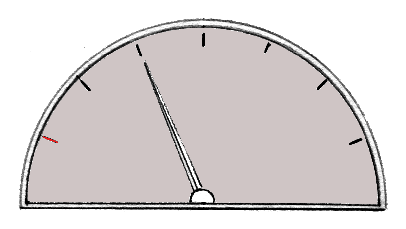
\includegraphics[width=3.7cm]{vitesse_matin}
 \begin{center} le matin \end{center}
 \end{minipage} \hfill%
 \begin{minipage}[c]{0.48\linewidth}
 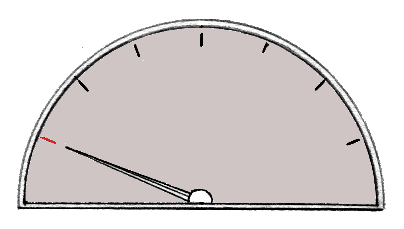
\includegraphics[width=3.7cm]{vitesse_soir}
 \begin{center} le soir \end{center}
  \end{minipage}
Sachant que le circuit journalier de l'employé fait 40 km, détermine si les soupçons de l'employeur sont justifiés.
\end{exercice}


\begin{exercice}[Farandole de fractions]
\begin{enumerate}
 \item On considère les fractions suivantes : \label{NbsRatio_approf20}
  \vspace{0.2cm} 
 \begin{center} $\dfrac{1}{2}$ ; $\dfrac{2}{3}$ ; $\dfrac{3}{4}$ ; $\dfrac{4}{5}$ ; \ldots \end{center}
 \begin{itemize}
  \item Complète cette suite logique avec trois autres fractions.
  \item Ces fractions sont-elles plus petites ou plus grandes que 1 ? Justifie.
  \item À l'aide de ta calculatrice, indique si ces fractions sont rangées dans l'ordre croissant ou décroissant.
  \end{itemize}
 \item On considère les fractions suivantes : \label{NbsRatio_approf21}
  \vspace{0.2cm} 
  \begin{center} $\dfrac{3}{2}$ ; $\dfrac{4}{3}$ ; $\dfrac{5}{4}$ ; $\dfrac{6}{5}$ ; \ldots \end{center}
 \begin{itemize}
  \item Complète cette suite logique avec trois autres fractions.
  \item Ces fractions sont-elles plus petites ou plus grandes que 1 ? Justifie.
  \item À l'aide de ta calculatrice, indique si ces fractions sont rangées dans l'ordre croissant ou décroissant.
  \end{itemize}
 \item En écrivant les fractions sous forme décimale (on arrondira au centième près quand c'est nécessaire), que remarques-tu pour les deux suites données en \ref{NbsRatio_approf20} et \ref{NbsRatio_approf21} ?
 \end{enumerate}
\end{exercice}


\begin{exercice}
Dans le but de faire du béton, Antoine a préparé (avant d'incorporer l'eau) un mélange de 100 kg composé de 30 \% de graviers, de trois huitièmes de sable et le reste de ciment. \\[0.5em]
Calcule la masse de chaque composant de ce mélange.
\end{exercice}


\begin{exercice}[La course]
Une course de 4\,500 m est organisée autour du collège. Durant cette course :
\begin{itemize}
 \item Ahmed doit stopper après avoir parcouru un dixième du trajet ;
 \item Bernard s'essouffle au bout des cinq sixièmes de la course ;
 \item Carolina, elle, n'atteint que le un quart de la longueur du parcours ;
 \item Dieter se blesse alors qu'il ne lui restait plus qu'un quinzième de la course à effectuer.
 \end{itemize}
Calcule la distance parcourue par chacun.
\end{exercice}


\begin{exercice}[Le club Ludimaths]
Un collège comporte 840 élèves dont les huit dixièmes sont demi‑pensionnaires. \\[0.5em]
Les sept douzièmes d'entre eux mangent au premier service, les autres au second service. Le club de jeux mathématiques a lieu durant le premier service et accueille un septième des élèves disponibles à ce moment-là.
\begin{enumerate}
 \item Combien d'élèves participent à ce club ?
 \item Quelle fraction du nombre total d'élèves représentent‑ils ? Simplifie‑la, si possible.
 \end{enumerate}
\end{exercice}


\begin{exercice}[Les soldes]
\begin{enumerate}
 \item Un article coûtant 30 CHF subit une première réduction de 50 \%. Calcule son nouveau prix.
 \item Lors d'une seconde démarque, le même article subit une nouvelle réduction de 50 \%.
 
Calcule son nouveau prix.
 \item Le prix de cet article a‑t‑il diminué de 100 \% après ces deux démarques ? Justifie.
 \end{enumerate}
\end{exercice}


\begin{exercice}[Le concours]
Un concours se déroule en deux étapes : 
\begin{itemize}
 \item tous les candidats passent les épreuves d'admissibilité à l'écrit ;
 \item seuls ceux qui sont déclarés "admissibles" passent les épreuves d'admission à l'oral. Ces derniers sont alors déclarés "admis" ou pas.
 \end{itemize}
1\,200 candidats se sont présentés à ce concours. Après l'écrit, un tiers d'entre eux a été recalé. Le reste a passé l'oral où les trois quarts n'ont finalement pas été admis. \\[0.5em]
Combien de candidats ont été admis à ce concours ?
\end{exercice}


\begin{exercice}[La marée]
Il est midi à Dunkerque et la marée est basse. La « règle des douzièmes » nous dit que la mer va monter de $\dfrac{1}{12}$ de l'amplitude totale pendant la première heure, de $\dfrac{2}{12}$ durant la 2\up{e} heure, de $\dfrac{3}{12}$ la 3\up{e} heure, encore $\dfrac{3}{12}$ la 4\up{e} heure, $\dfrac{2}{12}$ la 5\up{e} heure pour finir avec le dernier douzième la 6\up{e} heure et arriver enfin à marée haute.

La mer redescend ensuite de la même manière suivant un cycle d'environ six heures. \\[0.5em]
Reproduis et complète le tableau suivant en sachant que l'amplitude totale est de 3,60 m.
\begin{center}
 \begin{tabularx}{\linewidth}{|c|*{6}{>{\centering\arraybackslash}X|}}
 \hline
 Heure & 12 h & 13 h & \ldots & 23 h & 24 h \\\hline
 Hauteur d'eau (m) & 0 & & & & \\\hline
 \end{tabularx}
 \end{center}
\end{exercice}


\begin{exercice}[Le jardin]
Dans un terrain de 3,5 ha, les $\dfrac{4}{5}$ de la surface sont occupés par des arbres fruitiers. Les pommiers occupent les $\dfrac{2}{7}$ de la surface occupée par les arbres fruitiers. \\[0.2em]
Calcule, en m\up{2}, la surface occupée par les pommiers. (1 ha = 1 hm\up{2})
\end{exercice}


\begin{exercice}[Club sportif]
Le diagramme suivant donne la répartition des adhérents d'un club sportif selon leur sexe et selon leur tranche d'âge.
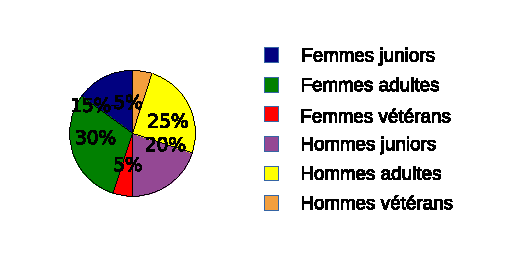
\includegraphics[width=8cm]{sport_stat}
\begin{enumerate}
 \item Reporte ces indications dans un tableau en remplaçant les pourcentages par des fractions simplifiées.
 \item Le club comporte 360 adhérents. Calcule le nombre d'adhérents de chaque catégorie.
 \end{enumerate}
\end{exercice}


\begin{exercice}[Triangle de Sierpinski]
Étapes de construction :
\begin{itemize}
 \item \underline{Étape 1} : On construit un triangle équilatéral qu'on prend pour unité d'aire.
 \item \underline{Étape 2} : On trace les trois segments joignant les milieux des côtés du triangle et on enlève le petit triangle central. Il reste trois petits triangles qui se touchent par leurs sommets et dont les longueurs des côtés sont la moitié de celles du triangle de départ.
 \item \underline{Étape 3} : On répète la deuxième étape avec chacun des petits triangles obtenus.
 \item \underline{Étapes suivantes} : On répète le processus.
 \end{itemize}
\begin{center} 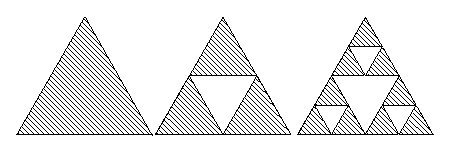
\includegraphics[width=7.5cm]{sierpinski_ratio} \end{center}
\begin{enumerate}
 \item Construis sur ton cahier les triangles obtenus aux étapes 3 et 4 (on prendra 8 cm de côté pour le triangle équilatéral de départ).
 \item Quelle fraction d'aire représente la partie hachurée, obtenue aux étapes 1, 2 et 3 ?
 \item Même question pour l'étape 4, de deux façons différentes : en regardant le schéma puis en faisant un calcul.
 \item Sans construire le triangle, indique quelle fraction d'aire la partie hachurée représente à l'étape 5.
 \item Et pour l'étape 8 ?
 \end{enumerate}
\end{exercice}

